\documentclass[border=2pt]{standalone}
\usepackage[T1]{fontenc}
\usepackage{lmodern}
\usepackage{pgfplots}
\pgfplotsset{compat=1.18}
\begin{document}
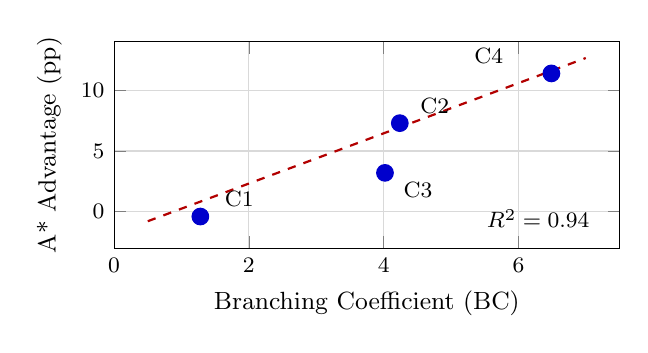
\begin{tikzpicture}
\begin{axis}[
    width=8cm,
    height=4.2cm,
    xlabel={Branching Coefficient (BC)},
    ylabel={A* Advantage (pp)},
    xmin=0, xmax=7.5,
    ymin=-3, ymax=14,
    grid=major,
    grid style={gray!30},
    tick label style={font=\footnotesize},
    label style={font=\small},
]
\addplot[only marks, mark=*, mark size=3pt, blue!80!black] coordinates {
    (1.28, -0.4)
    (4.24, 7.3)
    (4.02, 3.2)
    (6.49, 11.4)
};
\addplot[domain=0.5:7, samples=2, red!70!black, thick, dashed] {-1.82 + 2.07*x};
\node[font=\footnotesize, anchor=south west] at (axis cs:1.5,-0.4) {C1};
\node[font=\footnotesize, anchor=south west] at (axis cs:4.4,7.3) {C2};
\node[font=\footnotesize, anchor=north west] at (axis cs:4.15,3.2) {C3};
\node[font=\footnotesize, anchor=south west] at (axis cs:5.2,11.4) {C4};
\node[font=\footnotesize, anchor=north east] at (axis cs:7.2,1) {$R^2 = 0.94$};
\end{axis}
\end{tikzpicture}
\end{document}
